\chapter{Measurements}\label{ch:measurements}

\section{Recordings}

The measurements were conducted in an anechoic chamber at DTU's Department of Electrical Engineering using a microphone placed one meter away from the struck object. To record the sounds we used Bruel \& Kjær's half inch pressure field microphone type 4192 and microphone preamplifier power supply type 5935L, as well as the 744T digital audio recorder from Sound Devices at 44100 Hz sampling frequency. The setup can be seen in figure \ref{fig:experiment}.

\begin{figure}[H]
  \centering
    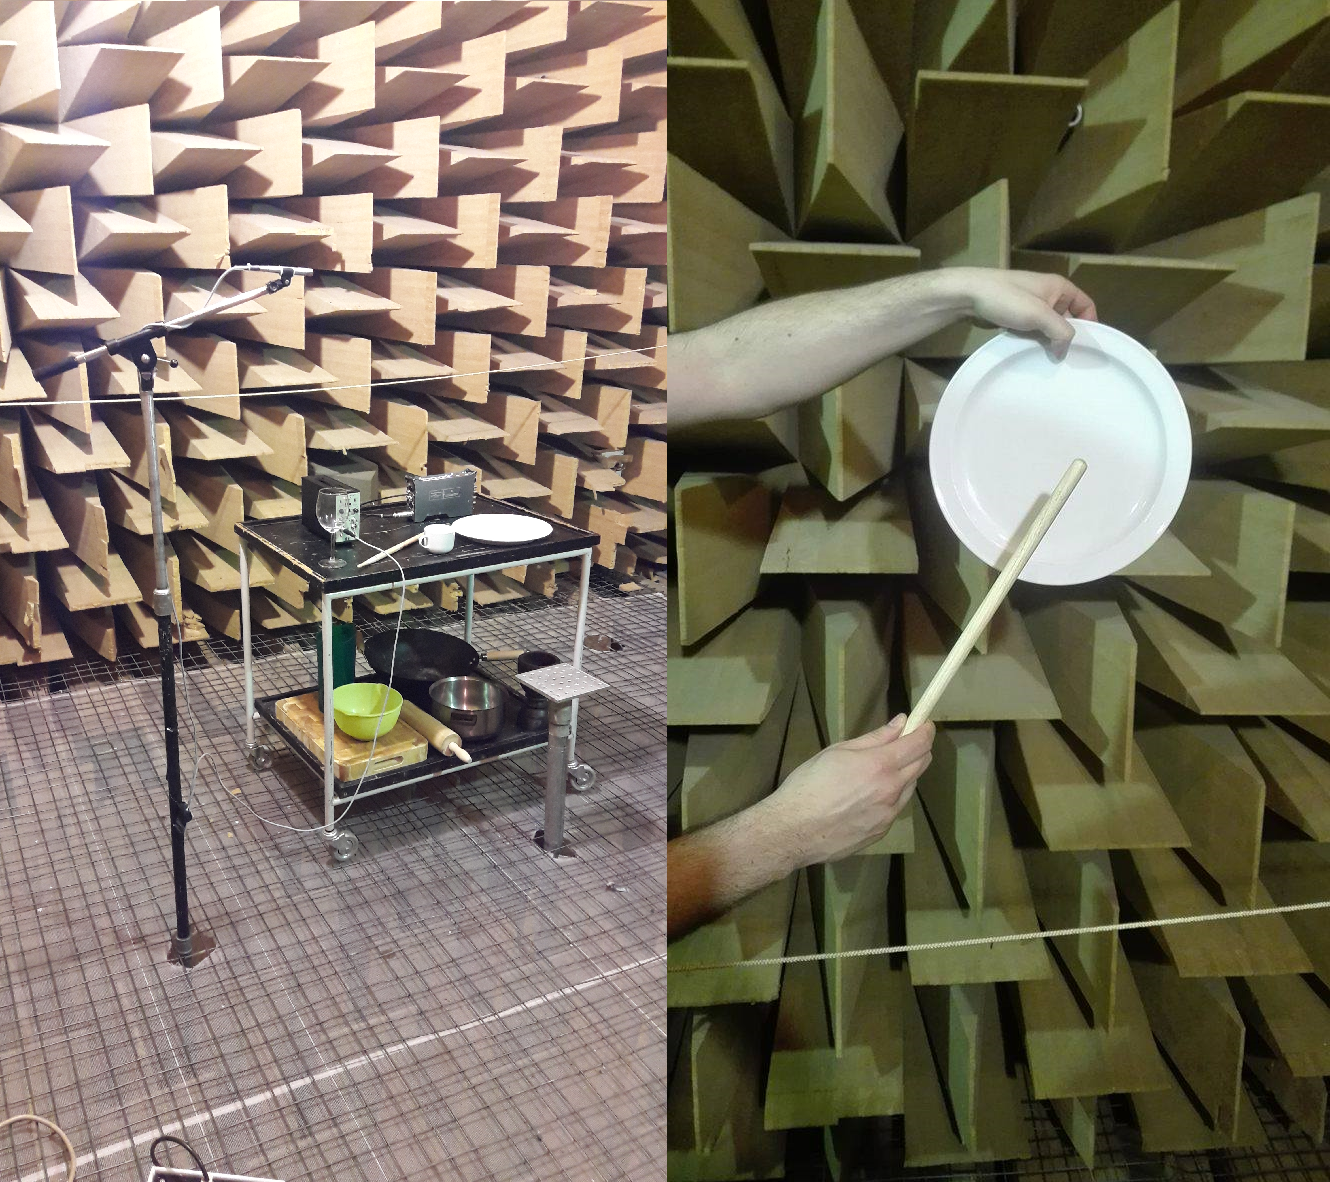
\includegraphics[width=0.6\textwidth]{experimentpic.png}
      \caption{Picture of the setup for the measurements (left) and of a struck object (right).}\label{fig:experiment}
\end{figure}

To control the impact we hit the objects by hand with a wooden drumstick (figure \ref{fig:experiment}) while trying to use the same impulsive force. Prior to the recordings, every object was divided into different surface areas depending on its shape and the sound produced by these areas. Therefore, several impact locations were chosen and recorded for every objects.

Eleven objects of everyday life made of five different materials (plastic, wood, ceramic, glass and metal) were used for the experiment. The idea of choosing these objects came firstly from the need of owning them (to perform the recording) and our ability to model them for the demo (as they should be simple enough). Secondly, since we wished to test the immersion of the synthesized sounds on users, we wanted to be sure that the sounds used are familiar to them. In figure \ref{fig:objects} both real and modeled objects are shown. 

\begin{figure}[H]
    \centering
    \begin{subfigure}[b]{0.7\textwidth}
        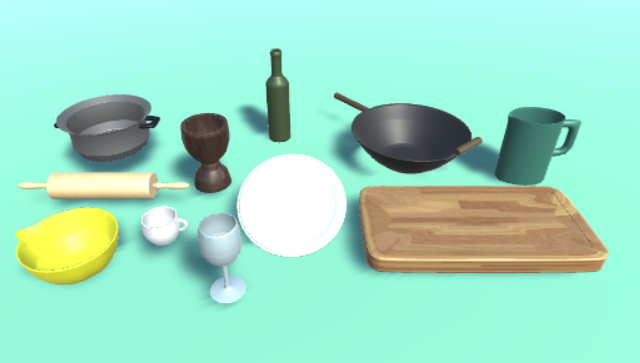
\includegraphics[width=\textwidth]{realobjects.PNG}
        \caption{Real objects.}
        \label{fig:gull}
    \end{subfigure}
    ~ %add desired spacing between images, e. g. ~, \quad, \qquad, \hfill etc. 
      %(or a blank line to force the subfigure onto a new line)
    \begin{subfigure}[b]{0.7\textwidth}
        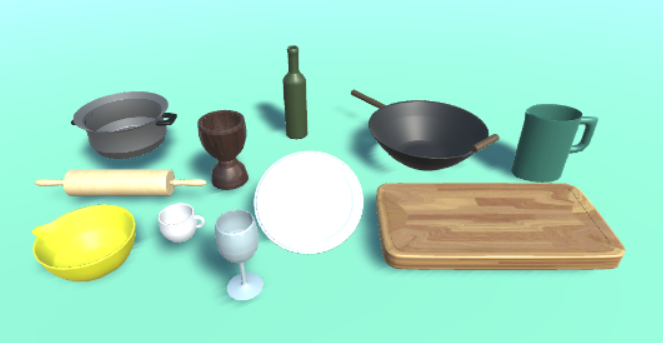
\includegraphics[width=\textwidth]{3dobjects.PNG}
        \caption{3D models of the objects.}
        \label{fig:tiger}
    \end{subfigure}
    \caption{The eleven objects used in the thesis.}\label{fig:objects}
\end{figure}

\section{User tests}

To examine the immersion of real-time produced and physics-based sounds on game players, we performed some \textit{MUSHRA} tests to people. By doing these tests we wanted to examine firstly which of the two synthesize methods is closer to reality and secondly the range of every material's sound.

\subsection{Stimuli}
We performed two different tests. The stimuli of the first one was 44 pairs of sounds (one for each synthesize method) corresponding to different areas of the eleven materials and their corresponding reference sounds which were the recordings of the actual sounds produce by the physical objects. The stimuli of the second test was 75 sounds coming from five different objects, one of each material under testing (plastic jug, wooden cutting board, ceramic plate, glass bottle and metallic cooking pot). For each of the objects, we used 15 different sounds which corresponded to a small variation on the Q-factor which changes the material of the object. More specifically, starting from a value of 600, we increased the Q-factor by 200 up to 4600 \Todo{check the numbers again} and provided participants with the produced sound.

In the first test, participants where provided with a reference sound (the actual recording) and two testing sounds (the sinusoidal and filter-based synthesized sounds), and were asked to choose the one sounding closer to the reference. In the second test, they were provided with sounds from the same object but with different materials assigned to it and they were asked to point out when a change in material happens. 

Sound starts 1sec after participant presses play.
\begin{itemize}
\item Recordings with different sound in every point area
\item Recordings with single sound per object\\
We picked the recording whose sound was closer to the real sound of this object in our opinion.\\

\end{itemize}

\subsection{Procedure}
Stimuli was presented to the participants through \Todo{describe headphones}, in a room with reduced external noise.

\subsection{Participants}
\Todo{number of participants, age, gender, normal hearing, job}